\documentclass[10pt,fleqn]{article} % Default font size and left-justified equations
\usepackage[%
    pdftitle={Modélisation systèmes multiphysiques : Modélisation linéaire et non linéaire},
    pdfauthor={Xavier Pessoles}]{hyperref}
    
\input{style/new_style}
%%%%%%%%%%%%
% Définition des vecteurs 
%%%%%%%%%%%%

\newcommand{\vect}[1]{\overrightarrow{#1}}
\newcommand{\axe}[2]{\left(#1,\vect{#2}\right)}
\newcommand{\couple}[2]{\left(#1,\vect{#2}\right)}
\newcommand{\angl}[2]{\left(\vect{#1},\vect{#2}\right)}

\newcommand{\rep}[1]{\mathcal{R}_{#1}}
\newcommand{\bas}[1]{\mathcal{B}_{#1}}
\newcommand{\quadruplet}[4]{\left(#1;#2,#3,#4 \right)}
\newcommand{\repere}[4]{\left(#1;\vect{#2},\vect{#3},\vect{#4} \right)}
\newcommand{\base}[3]{\left(\vect{#1},\vect{#2},\vect{#3} \right)}


\newcommand{\vx}[1]{\vect{x_{#1}}}
\newcommand{\vy}[1]{\vect{y_{#1}}}
\newcommand{\vz}[1]{\vect{z_{#1}}}
\newcommand{\vi}[1]{\vect{i_{#1}}}
\newcommand{\vj}[1]{\vect{j_{#1}}}
\newcommand{\vk}[1]{\vect{k_{#1}}}
\newcommand{\vAB}{\vect{AB}}
\newcommand{\vBA}{\vect{BA}}
\newcommand{\vBC}{\vect{BC}}
\newcommand{\vCB}{\vect{CB}}
\newcommand{\vCA}{\vect{CA}}
\newcommand{\vAC}{\vect{AC}}


% d droit pour le calcul différentiel
\newcommand{\dd}{\text{d}}
\newcommand{\deriv}[2]{ \dfrac{ \dd }{\dd t} \left[  #1\right]_{#2}}
\newcommand{\dderiv}[2]{ \dfrac{ \dd^2 }{\dd t^2} \left[  #1\right]_{#2}}

% dérivée
\newcommand{\varphip}{\dot{\varphi}}
\newcommand{\thetap}{\dot{\theta}}
\newcommand{\lambdap}{\dot{\lambda}}
\newcommand{\varphipp}{\ddot{\varphi}}
\newcommand{\thetapp}{\ddot{\theta}}
\newcommand{\lambdapp}{\ddot{\lambda}}



\newcommand{\inertie}[2]{I_{#1}\left( #2\right)}
\newcommand{\matinertie}[7]{
\begin{pmatrix}
#1 & #6 & #5 \\
#6 & #2 & #4 \\
#5 & #4 & #3 \\
\end{pmatrix}_{#7}}
%%%%%%%%%%%%
% Définition des torseurs 
%%%%%%%%%%%%

\newcommand{\ec}[2]{%
\mathcal{E}_c\left(#1/#2\right)}

\newcommand{\pext}[3]{%
\mathcal{P}\left(#1\rightarrow#2/#3\right)}

\newcommand{\pint}[3]{%
\mathcal{P}\left(#1 \stackrel{\text{#3}}{\leftrightarrow} #2\right)}


 \newcommand{\torseur}[1]{%
\left\{{#1}\right\}
}

\newcommand{\torseurcin}[3]{%
\left\{\mathcal{#1} \left(#2/#3 \right) \right\}
}

\newcommand{\torseurci}[2]{%
%\left\{\sigma \left(#1/#2 \right) \right\}
\left\{\mathcal{C} \left(#1/#2 \right) \right\}
}
\newcommand{\torseurdyn}[2]{%
\left\{\mathcal{D} \left(#1/#2 \right) \right\}
}


\newcommand{\torseurstat}[3]{%
\left\{\mathcal{#1} \left(#2\rightarrow #3 \right) \right\}
}


 \newcommand{\torseurc}[8]{%
%\left\{#1 \right\}=
\left\{
{#1}
\right\}
 = 
\left\{%
\begin{array}{cc}%
{#2} & {#5}\\%
{#3} & {#6}\\%
{#4} & {#7}\\%
\end{array}%
\right\}_{#8}%
}

 \newcommand{\torseurcol}[7]{
\left\{%
\begin{array}{cc}%
{#1} & {#4}\\%
{#2} & {#5}\\%
{#3} & {#6}\\%
\end{array}%
\right\}_{#7}%
}

 \newcommand{\torseurl}[3]{%
%\left\{\mathcal{#1}\right\}_{#2}=%
\left\{%
\begin{array}{l}%
{#1} \\%
{#2} %
\end{array}%
\right\}_{#3}%
}

% Vecteur vitesse
\newcommand{\vectv}[3]{%
\vect{V\left( {#1} , {#2}/{#3}\right)}
}

% Vitesse du point
\newcommand{\vectvp}[2]{%
\vect{V\left( {#1} /{#2}\right)}
}

% Vecteur force
\newcommand{\vectf}[2]{%
\vect{R\left( {#1} \rightarrow {#2}\right)}
}

% Vecteur moment stat
\newcommand{\vectm}[3]{%
\vect{\mathcal{M}\left( {#1}, {#2} \rightarrow {#3}\right)}
}




% Vecteur résultante cin
\newcommand{\vectrc}[2]{%
\vect{R_c \left( {#1}/ {#2}\right)}
}
% Vecteur moment cin
\newcommand{\vectmc}[3]{%
\vect{\sigma \left( {#1}, {#2} /{#3}\right)}
}


% Vecteur résultante dyn
\newcommand{\vectrd}[2]{%
\vect{R_d \left( {#1}/ {#2}\right)}
}
% Vecteur moment dyn
\newcommand{\vectmd}[3]{%
\vect{\delta \left( {#1}, {#2} /{#3}\right)}
}

% Vecteur accélération
 \newcommand{\vectg}[3]{%
\vect{\Gamma \left( {#1}, {#2}/{#3}\right)}
}
% Vecteur accélération du point
 \newcommand{\vectgp}[2]{%
\vect{\Gamma \left( {#1}/{#2}\right)}
}

% Vecteur omega
 \newcommand{\vecto}[2]{%
\vect{\Omega\left( {#1}/{#2}\right)}
}
% }$$\left\{\mathcal{#1} \right\}_{#2} =%
% \left\{%
% \begin{array}{c}%
%  #3 \\%
%  #4 %
% \end{array}%
% \right\}_{#5}}

%Varignon dynamique
 \newcommand{\babard}[4]{%
\vectmd{#1}{#3}{#4}=\vectmd{#2}{#3}{#4}+\vect{#1#2}\wedge \vectrd{#3}{#4}
}

%Varignon cinématique
 \newcommand{\babarv}[4]{%
\vectv{#1}{#3}{#4}=\vectv{#2}{#3}{#4}+\vect{#1#2}\wedge \vecto{#3}{#4}
}

%% SLCI
% Ordre 1
\newcommand{\ordreun}{\dfrac{K}{1+\tau p}}

\newcommand{\ordreunopt}[2]{\dfrac{#1}{1+#2 p}}
% Ordre 2
\newcommand{\ordredeux}{\dfrac{K}{1+\dfrac{2\xi}{\omega_0}p+\dfrac{p^2}{\omega_0^2}}}

% MCC
\newcommand{\mccel}{U(t)=E(t)+RI(t)+L\dfrac{\dd i(t)}{\dd t}}
%\newcommand{\mccmeca}{J \dfrac{\dd \omega(t)}{\dd t}=C }




%Binaire, octal, hexa
\newcommand{\hex}[1]{\underline{\text{\texttt{#1}}}_{16}}
\newcommand{\oct}[1]{\underline{\text{\texttt{#1}}}_{8}}
\newcommand{\bin}[1]{\underline{\text{\texttt{#1}}}_{2}}


% Fonctions et systèmes
\usepackage{multicol}
\usepackage{standalone}
\standaloneconfig{mode=buildnew}
\usepackage{siunitx}
\usepackage{wrapfig}
\usepackage{float}
\usepackage{listings}
\lstset{language=Python,
  inputencoding=utf8,
  breaklines=true,
  basicstyle=\ttfamily\small,
  keywordstyle=\bfseries\color{green!40!black},
  commentstyle=\itshape\color{purple!40!black},
  identifierstyle=\color{blue},
  stringstyle=\color{orange},
  upquote = true,
  columns=fullflexible,
  backgroundcolor=\color{gray!10},frame=leftline,rulecolor=\color{gray}}  
  
\definecolor{mygreen}{rgb}{0,0.6,0}


\lstset{
     literate=%
         {é}{{\'e}}1    
         {è}{{\`e}}1    
         {ê}{{\^e}}1    
         {à}{{\`a}}1    
         {ô}{{\^o}}1    
         {ù}{{\`u}}1    
}

\graphicspath{{images/}{png/}}

\fichetrue

%\fichefalse

\proftrue
\proffalse

\tdtrue
%\tdfalse

\courstrue
\coursfalse

\def\discipline{Sciences \\Industrielles de \\ l'Ingénieur}
\def\xxtete{Sciences Industrielles de l'Ingénieur}

\def\classe{PSI$\star$}
\def\xxnumpartie{{DS 1}}%\textsf{\textsf{Cy. 4, 6 \& 7}}}
\def\xxpartie{Devoir Surveillé 1}


\def\xxnumchapitre{20 septembre 2021 \vspace{.2cm} $\;$ }
\def\xxchapitre{\hspace{.12cm} Performances des systèmes asservis}


\def\xxtitreexo{\noindent Robot delta 2 axes de transfert dans une chaine}
\def\xxsourceexo{\hspace{.2cm} Centrale Supelec -- TSI 2020}


\def\xxposongletx{2}
\def\xxposonglettext{1.45}
\def\xxposonglety{20}
%\def\xxonglet{Part. 1 -- Ch. 3}
\def\xxonglet{\textsf{DS 1}}%\textsf{\textsf{Cy. 4, 6 \& 7}}}

\def\xxactivite{\textsf{DS 1}}
\def\xxauteur{\textsl{Xavier Pessoles}}

\def\xxcompetences{%
\textsl{%
%\textbf{Savoirs et compétences :}\\
%Les sources sont associées par un \emph{hacheur série}. La détermination des grandeurs électriques associées à ce montage permet de conclure vis à vis du cahier des charges.
%\noindent \textbf{Résoudre :} à partir des modèles retenus :
%\begin{itemize}[label=\ding{112},font=\color{ocre}] 
%\item choisir une méthode de résolution analytique, graphique, numérique;
%\item mettre en \oe{}uvre une méthode de résolution.
%\end{itemize}
%\begin{itemize}[label=\ding{112},font=\color{ocre}] 
%\item \textit{Rés -- C1.1 :} Loi entrée sortie géométrique et cinématique -- Fermeture géométrique.
%\end{itemize}
%
%\noindent \textit{Mod2 -- C4.1 :} Représentation par schéma-blocs.
}}

\def\xxfigures{
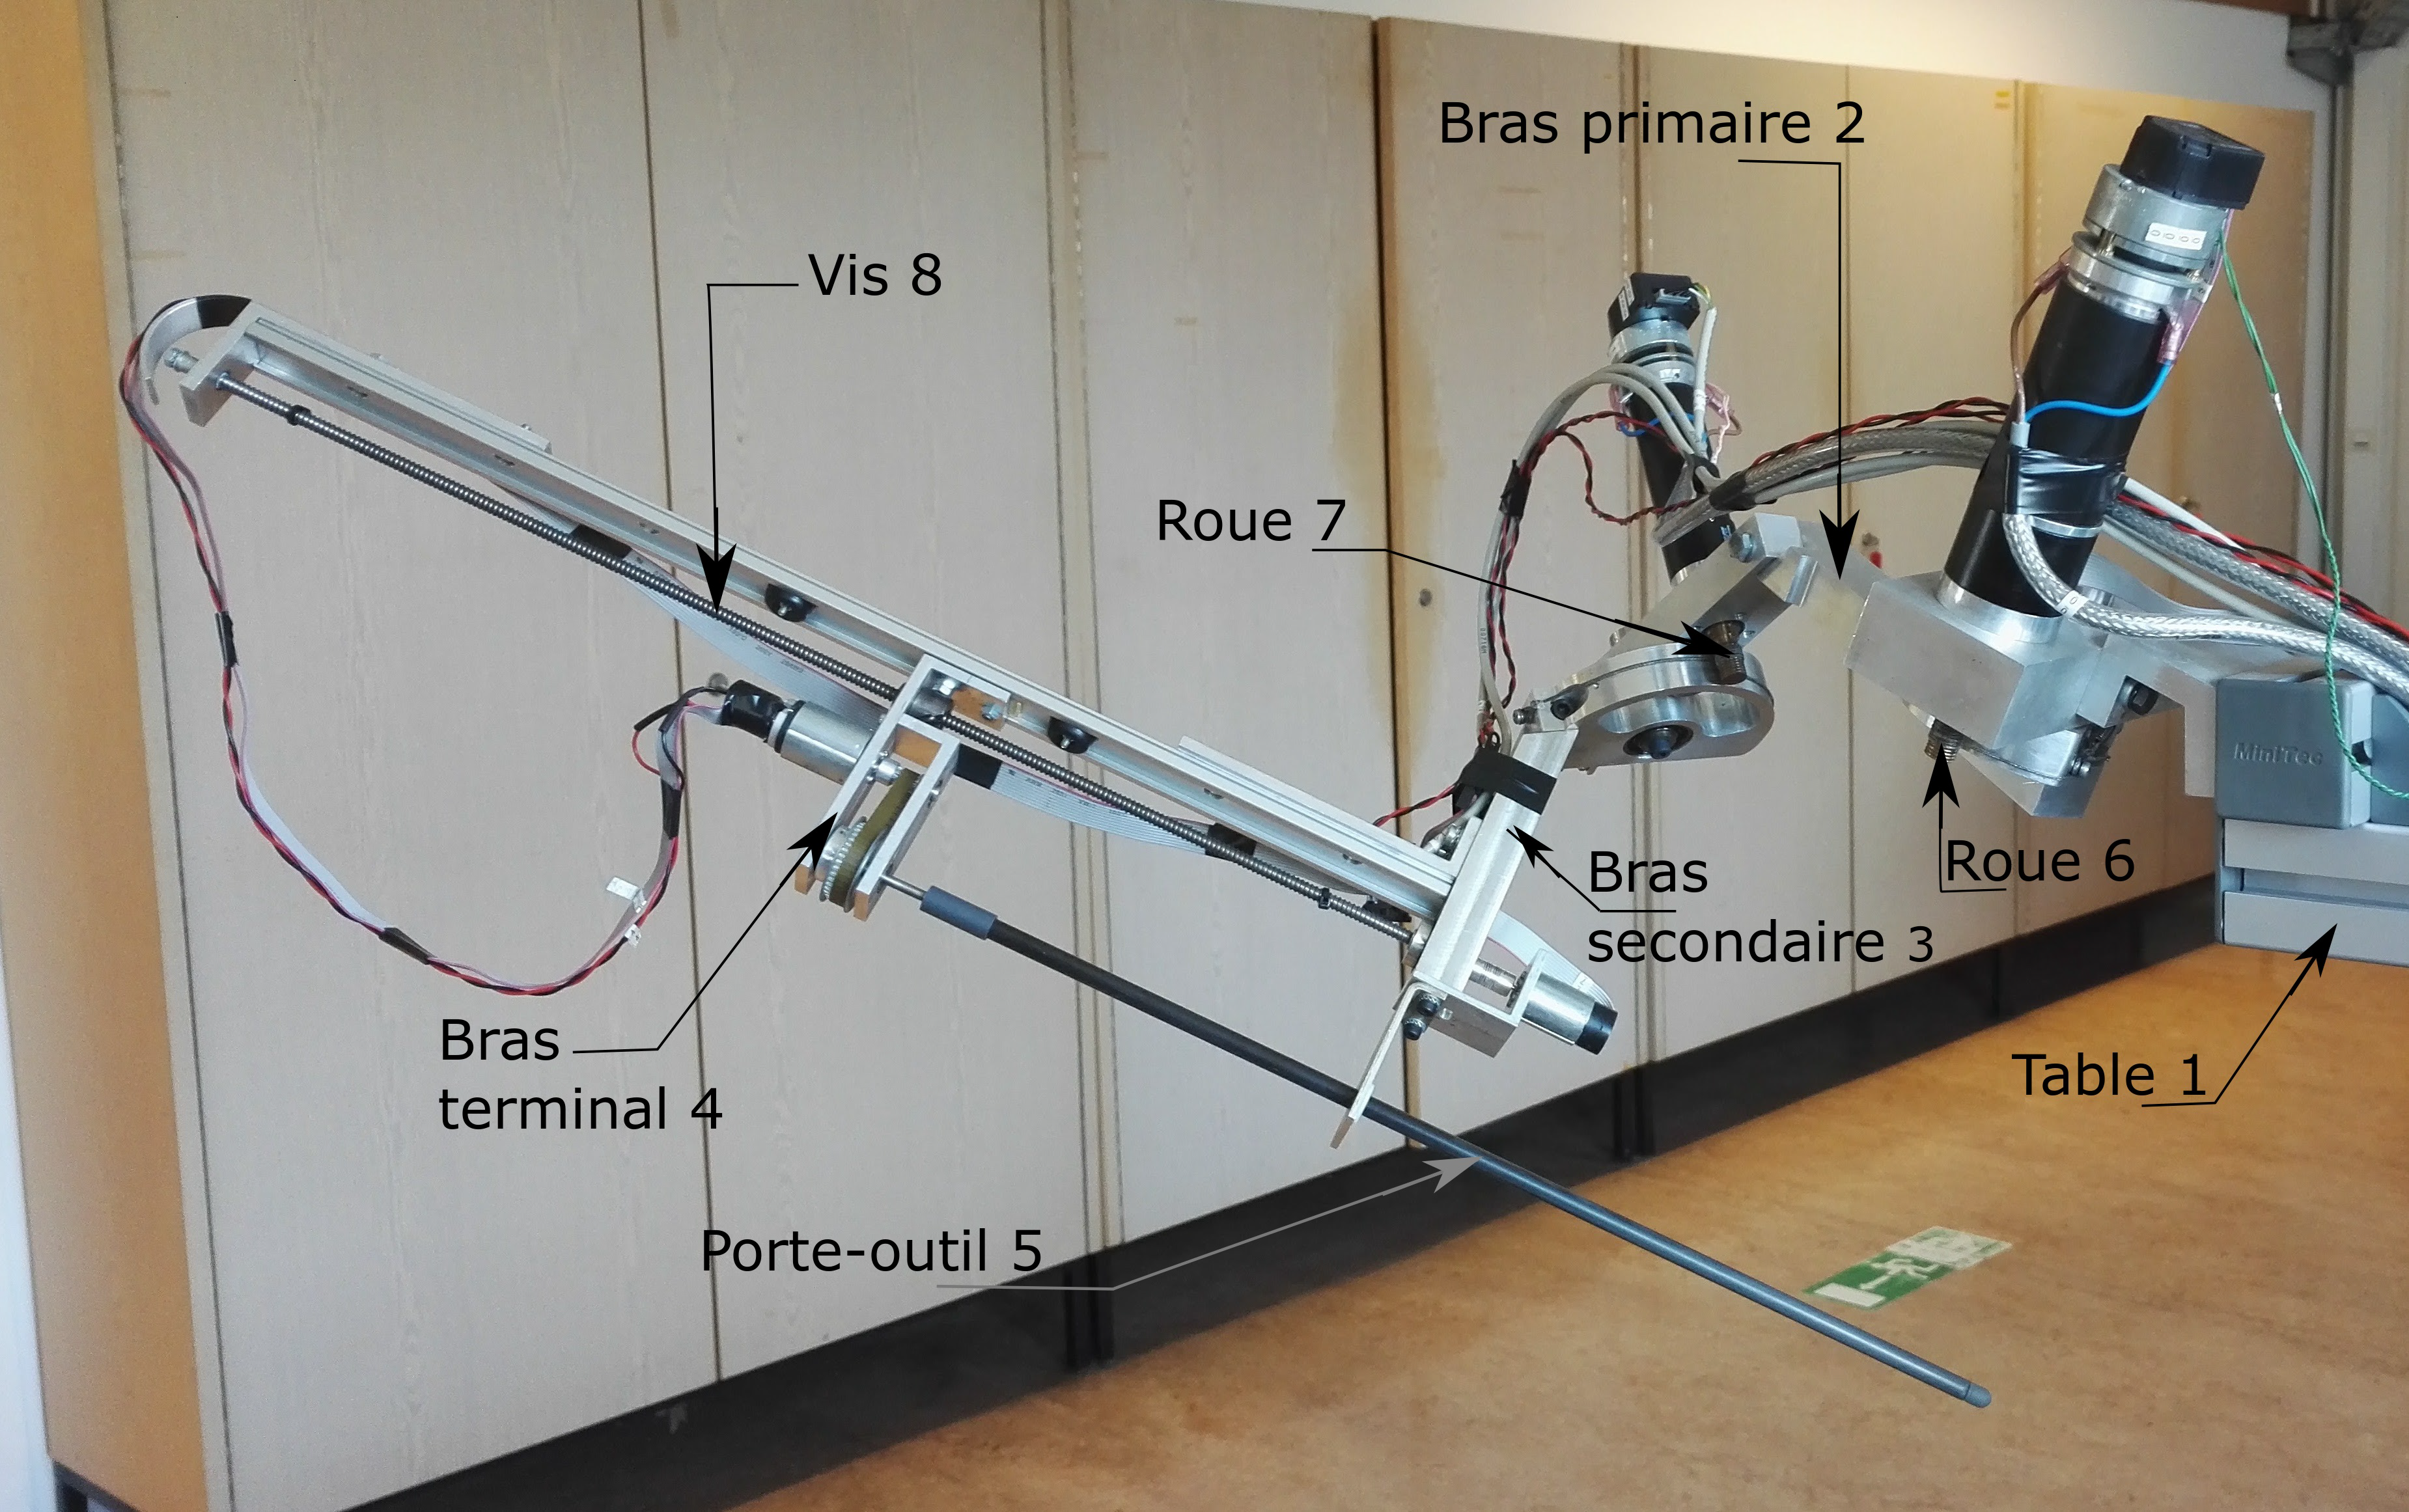
\includegraphics[width=.55\linewidth]{fig_00}
}%figues de la page de garde


\def\xxpied{%
%Cycle 01 -- Modéliser le comportement des systèmes multiphysiques\\
\xxactivite%
}

\setcounter{secnumdepth}{5}
%---------------------------------------------------------------------------

\usepackage{pgfplots}
\begin{document}
%\defimages{images}
%\chapterimage{png/Fond_Cin}
\input{style/new_pagegarde}
\vspace{4.5cm}
\pagestyle{fancy}
\thispagestyle{plain}

\def\columnseprulecolor{\color{ocre}}
\setlength{\columnseprule}{0.4pt} 

%\defimages2{images}

%\begin{multicols}{2}


\section{Présentation du système}

\ifprof
\else
L’étude concerne un robot de type « delta 2 axes » utilisé dans une usine de conditionnement de produits
agroalimentaires. Ce robot est destiné à remplacer un robot de type cartésien (mouvement vertical et horizontal)
utilisé pour un transfert rapide de produits emballés entre 2 tapis roulants. Plusieurs modèles de ce type de
robot sont commercialisés. L’étude porte sur celui présenté sur la figure 1.



\begin{figure}[H]
\centering
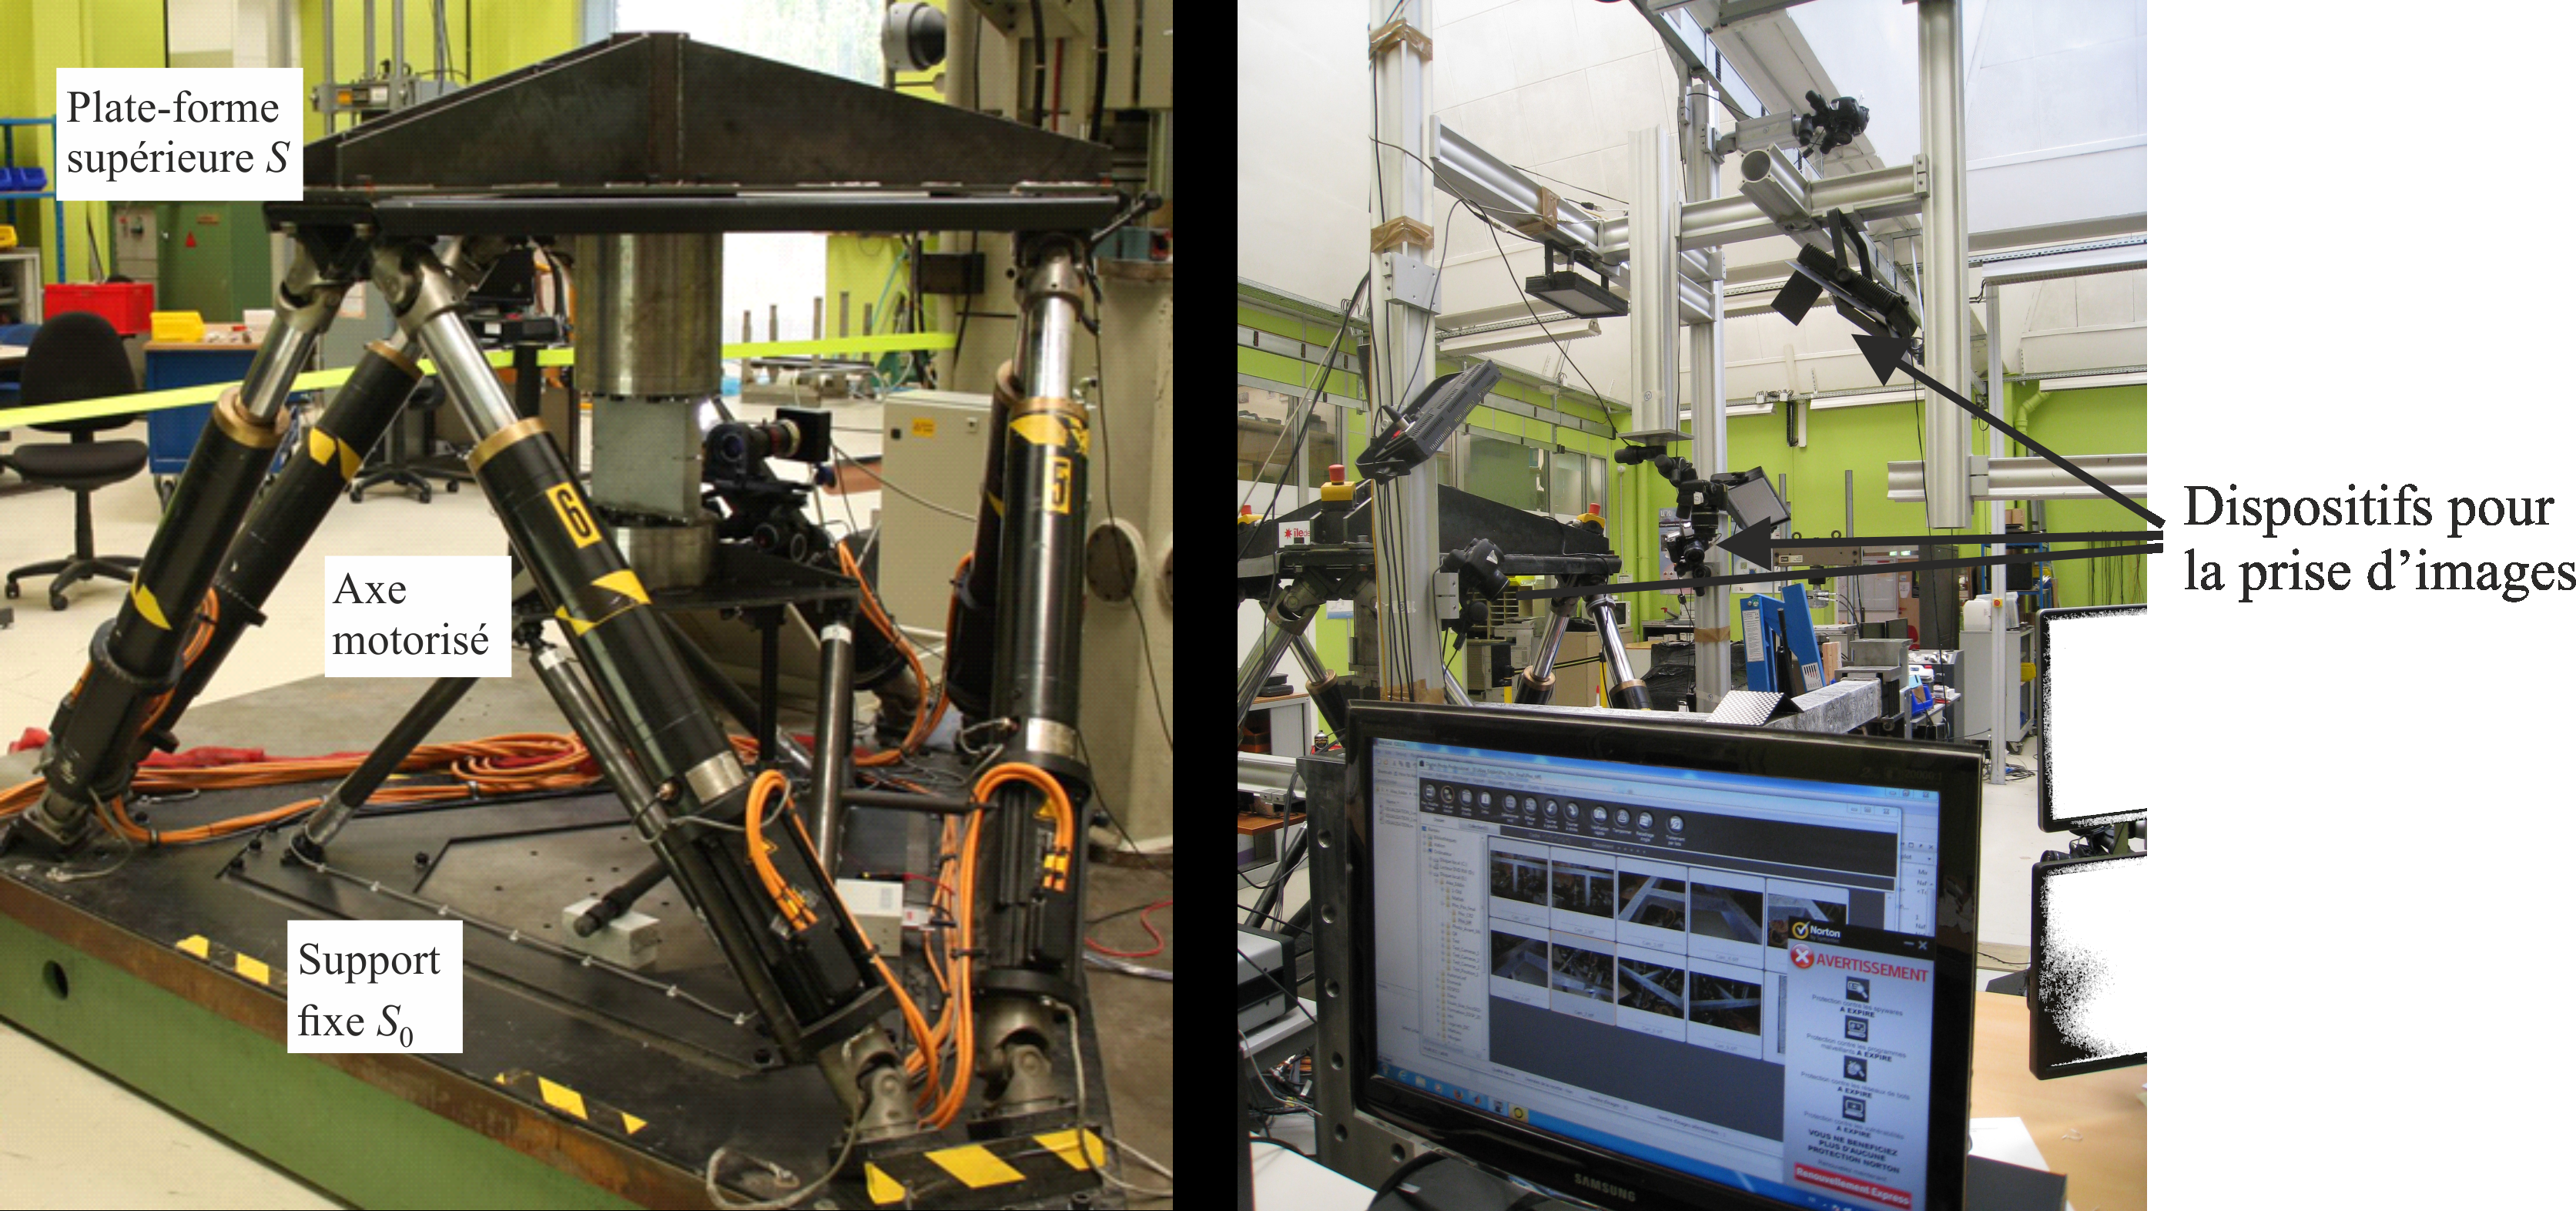
\includegraphics[width=0.9\linewidth]{fig_01}
\caption{Robot delta 2 axes \label{fig_01}}
\end{figure}




Le robot est mis en mouvement par deux moteurs synchrones à aimants permanents (figures 1 et 2). Chaque moteur
entraine un bras principal par l’intermédiaire d’un réducteur à train épicycloïdal. Les deux bras principaux
$bp_1$ et $bp_2$ sont en liaison pivot avec deux bras secondaires $bs_1$ et $bs_2$. Les deux bras secondaires (figure 3) sont
en liaison pivot avec le préhenseur. Un système à double parallélogramme permet de maintenir l’objet déplacé
dans un plan parallèle au sol. Les moteurs sont alimentés par des variateurs de vitesse dont les consignes de
vitesse sont issues d’une unité centrale de traitement.

Un codeur de position solidaire de l’axe moteur est utilisé pour le fonctionnement en mode synchrone autopiloté.
La position angulaire de chaque axe moteur est transmise à l’unité centrale par les variateurs.
L’exigence sur la précision de dépose entre les deux tapis roulants n’est pas très élevée ($\pm\SI{5}{mm}$). En aval du
tapis roulant sur lequel sont transférés les produits emballés se trouve un système d’impression. Afin de respecter
une bonne qualité d’impression pour chaque série identique de produits emballés, une exigence plus élevée est
requise pour la répétabilité du positionnement ($\pm\SI{0,1}{mm}$).
Ce robot doit remplir plusieurs exigences :
\begin{itemize}
\item « garantir le mouvement de translation », ce qui nécessite de dimensionner les moteurs synchrones du robot
en vitesse et en couple pour un mouvement donné ;
\item « fournir l’énergie électrique aux moteurs » afin que la source d’énergie alimentant l’ensemble des motovariateurs
permette le déplacement de la charge à soulever par le robot ;
\item « assurer une pose précise » en élaborant un programme de calcul d’incertitude de positionnement du préhenseur
à partir de la connaissance de la précision de positionnement angulaire des moteurs ;
\item « gérer le mouvement » en déterminant les paramètres de réglage de la commande asservie des moteurs
permettant d’assurer le déplacement requis.
\end{itemize}

\begin{figure}[H]
\centering
\includegraphics[width=\linewidth]{fig_02}
\caption{Diagramme de blocs internes partiel \label{fig_02}}
\end{figure}
\fi

\section{Exigence fonctionnelle « garantir le mouvement de translation »}

\begin{obj}
Proposer un modèle de connaissance des éléments réalisant l’exigence fonctionnelle « assurer le mouvement
de translation » puis valider les performances attendues listées par le cahier des charges (tableau
1).
\end{obj}

\ifprof
\else
\begin{center}
\includegraphics[width=\linewidth]{tab_01}

\textit{Tableau 1 -- Extrait du cahier des charges associé à l’exigence « garantir le mouvement de translation »}
\end{center}

\fi

\subsection{Élaboration du modèle articulaire inverse}
\begin{obj}
Élaborer la commande des moteurs à partir d’un mouvement défini dans l’espace opérationnel puis
converti dans l’espace articulaire.
\end{obj}
\ifprof
\else

Le schéma cinématique du robot est présenté figure 3. Un système à double parallélogramme permet de maintenir
l’objet déplacé dans un plan parallèle au sol. Pour la suite de l’étude, le schéma cinématique simplifié sera utilisé.

\subsubsection*{Hypothèse}
Le référentiel lié au repère $\rep{0}\left(O,\vect{x_0},\vect{y_0},\vect{z_0} \right)$ est galiléen et est fixe par rapport à la terre.
\subsubsection*{Données}
\begin{itemize}
\item $\left(\vect{x_0},\vect{x_1}\right)=\theta_{10}$, 
$\left(\vect{x_0},\vect{x_2}\right)=\theta_{20}$, 
$\left(\vect{x_0},\vect{x_3}\right)=\theta_{30}$, 
$\left(\vect{x_0},\vect{x_4}\right)=\theta_{40}$;
\item $\vect{OA}=a\vect{x_0}$, 
$\vect{OC}=-a\vect{x_0}$, 
$\vect{AB}=b\vect{x_1}$, 
$\vect{CD}=b\vect{x_2}$, 
$\vect{BE}=c\vect{x_3}$, 
$\vect{DE}=c\vect{x_4}$;
\item $a=\SI{150}{mm}$, $b=\SI{400}{mm}$, $c=\SI{850}{mm}$.
\end{itemize}

\fi
\subparagraph{\label{q_01}}\textit{Déterminer littéralement $\left(x_E,y_E\right)$, les composantes du vecteur $\vect{OE}$ correspondant à la position du
point $E$ appartenant à l’effecteur par rapport à $\rep{0}$, en fonction des coordonnées articulaires et $\theta_{10}$ et $\theta_{30}$ et des
paramètres dimensionnels $a$, $b$ et $c$. Exprimer ces coordonnées opérationnelles dans le repère $\rep{0}$.}
\ifprof
\begin{corrige}
On a $\vect{OE}=\vect{OA}+\vect{AB}+\vect{BE}$ donc $\vect{OE}=a\vect{x_0}+b\vect{x_1}+c\vect{x_3}$.

On projette ensuite $\vect{OE}$ dans $\rep{0}$.
$\vect{OE}=a\vect{x_0}+b\left(\cos\theta_{10}\vx{0}+\sin\theta_{10}\vy{0} \right)+c\left(\cos\theta_{30}\vx{0}+\sin\theta_{30}\vy{0} \right)$.

On a donc :
$
\left\{\begin{array}{l}
x_E = a+b\cos\theta_{10} +c\cos\theta_{30} \\
y_E =     b\sin\theta_{10}  +c\sin\theta_{30}
\end{array} \right.$ avec $\vect{OE}=x_E\vx{0}+y_E\vy{0}$. 

\end{corrige}
\else
\fi

Nous allons maintenant déterminer les coordonnées articulaires $\theta_{10}$ et $\theta_{30}$ en fonction des longueurs $x_E$, $y_E$, $a$, $b$ et $c$.

\subparagraph{\label{q_02}}\textit{À partir des deux relations scalaires trouvées à la question \ref{q_01}, provenant du modèle géométrique direct, établir une équation de la forme $A\cos\theta_{10}+ B\sin\theta_{10} = C$. On explicitera les $A$, $B$ et $C$.}


%exprimer $c \cos\theta_{30}$ et $c \sin\theta_{30}$ en fonction de $x_E$, $y_E$, $a$, $b$ et $\theta_{10}$}
\ifprof
\begin{corrige}
On en déduit d'abord que  
$
\left\{\begin{array}{l}
c\cos\theta_{30} = x_E - a-b\cos\theta_{10}\\
c\sin\theta_{30} = y_E -    b\sin\theta_{10}  
\end{array} \right.$

En élevant les expressions au carré puis en les sommant, on a 
$\left( c\cos\theta_{30} \right)^2 +\left( c\sin\theta_{30} \right)^2 =
\left(x_E - a-b\cos\theta_{10} \right)^2 + \left( y_E -    b\sin\theta_{10}\right)^2 $
soit 
$ c^2 = \left(x_E - a-b\cos\theta_{10} \right)^2 + \left( y_E -    b\sin\theta_{10}\right)^2 $.

En développant cette expression, on a alors 

$ c^2 = x_E^2 + a^2+b^2\cos^2\theta_{10}  
-2x_Ea- 2x_Eb\cos\theta_{10} + 2ab\cos\theta_{10}
+  y_E^2 +    b^2\sin^2\theta_{10} 
-2y_E   b\sin\theta_{10} $.

$\Longleftrightarrow c^2 = x_E^2 + a^2+b^2 -2x_Ea- 2x_Eb\cos\theta_{10} + 2ab\cos\theta_{10} +  y_E^2   -2y_E   b\sin\theta_{10} $

$\Longleftrightarrow c^2 - x_E^2 - a^2-b^2 +2x_Ea - y_E^2 = 2b\left(a- x_E\right) \cos\theta_{10}   -2y_E   b\sin\theta_{10} $.


On a donc :
$\left\{
\begin{array}{l}
A = 2b\left(a- x_E\right) \\
B =-2y_E   b \\
C = c^2 - x_E^2 - a^2-b^2 +2x_Ea - y_E^2 
\end{array}
\right.$


\end{corrige}
\else
\fi

\ifprof
\else

\begin{figure}[H]
\centering
\includegraphics[width=\linewidth]{fig_03}
\caption{Schémas cinématiques \label{fig_03}}
\end{figure}

\fi

%\subparagraph{\label{q_03}}\textit{En sommant les carrés des sinus et cosinus de l’angle $\theta_{30}$, établir une équation de la forme $A\cos\theta_{10}+ B\cos\theta_{10} = C$.}
%\ifprof
%\begin{corrige}
%\end{corrige}
%\else
%\fi

\subparagraph{\label{q_04}}\textit{Montrer alors qu’il est possible, en posant un angle $\varphi$  tel que 
$\tan \varphi = \dfrac{A}{B}$, d’écrire cette équation sous la forme $\sin\left(\theta_{10}+\varphi \right)=\dfrac{C}{\sqrt{A^2 + B^2}}$.}
\ifprof
\begin{corrige}
Commençons par diviser l'équation obtenue précédemment par $\sqrt{A^2 + B^2}$ : 

 $\dfrac{A}{\sqrt{A^2 + B^2}}\cos\theta_{10}+ \dfrac{B}{\sqrt{A^2 + B^2}}\cos\theta_{10} = \dfrac{C}{\sqrt{A^2 + B^2}}$. 
 
 Par ailleurs, on pose   $\sin\varphi = \dfrac{A}{\sqrt{A^2 + B^2}}\cos\theta_{10}$ et 
 $\cos\varphi = \dfrac{B}{\sqrt{A^2 + B^2}}\cos\theta_{10}$. On a alors $\tan \varphi = \dfrac{A}{B}$.
 
 On a donc    $\sin\varphi \cos\theta_{10}+ \cos\varphi \cos\theta_{10} = \dfrac{C}{\sqrt{A^2 + B^2}}$. 

Or $ \sin\theta_{10} \cos\varphi + \sin\varphi  \cos\theta_{10}=\sin\left(\theta_{10}+\varphi \right)  $; donc
  $\sin\left(\theta_{10}+\varphi \right) =  \dfrac{C}{\sqrt{A^2 + B^2}}$.
 

\end{corrige}
\else
\fi

\subparagraph{\label{q_05}}\textit{Exprimer $\theta_{10}$ en fonction des coefficients $A$, $B$ et $C$ puis en fonction des grandeurs du texte.}
\ifprof
\begin{corrige}

On a $\theta_{10}+\varphi  = \arcsin\left( \dfrac{C}{\sqrt{A^2 + B^2}}\right)$
soit $\theta_{10}  = \arcsin\left( \dfrac{C}{\sqrt{A^2 + B^2}}\right)  - \arctan\left(\dfrac{A}{B}\right)$.

En utilisant le changement de variable, on a 

$\theta_{10}  = \arcsin\left( \dfrac{ c^2 - x_E^2 - a^2-b^2 +2x_Ea - y_E^2}{\sqrt{\left( 2b\left(a- x_E\right)\right)^2 + \left( -2y_E   b  \right)^2}}\right)  - \arctan\left(\dfrac{\left( 2b\left(a- x_E\right)\right)}{\left( -2y_E   b  \right)}\right)$

soit 
$\theta_{10}  = \arcsin\left( \dfrac{ c^2 - x_E^2 - a^2-b^2 +2x_Ea - y_E^2}{2b\sqrt{\left( a- x_E\right)^2 +  y_E   ^2}}\right)  - \arctan\left(\dfrac{  x_E-a}{ y_E  }\right)$.

\end{corrige}
\else
\fi

\subparagraph{\label{q_06}}\textit{Déterminer l’expression de $\theta_{30}$ à partir d’une des deux relations trouvées à la question 1.}
\ifprof
\begin{corrige}

On a   $y_E =    b\sin\theta_{10}  +c\sin\theta_{30}$; donc 
 $ \sin\theta_{30} =\dfrac{ y_E -  b\sin\theta_{10}}{c} $. 
 
\end{corrige}
\else
\fi

\ifprof
\else

Une étude similaire permet d’établir également les expressions des coordonnées articulaires $\theta_{20}$ et $\theta_{40}$.
\fi

\subsection{Élaboration du modèle dynamique}

\begin{obj}
Dimensionner les moteurs du robot. Ces calculs visent à déterminer l’équation dynamique qui permet
d’obtenir le couple moteur minimal en fonction de la masse de la charge à soulever.
\end{obj}

\ifprof
\else

\subsubsection*{Hypothèses}
\begin{itemize}
\item L’étude est modélisable dans le plan.
\item Toutes les liaisons sont parfaites (au sens énergétique) donc sans jeu ni frottement.
\item Les inerties et les masses des pièces sont négligées, sauf la masse $m$ de la charge à soulever et l’inertie du rotor du moteur autour de son axe de rotation notée $J_m$.
\end{itemize}

Les différentes actions mécaniques sont :
$\torseurstat{T}{\text{réducteur 1}}{\text{bp}_1} = \torseurl{\vect{0}}{C_1\vect{z_0}}{A}$,
$\torseurstat{T}{\text{pesanteur}}{\text{charge}} = \torseurl{-mg\vect{y_0}}{\vect{0}}{E}$,
$\torseurstat{T}{\text{bs}_1}{\text{préhenseur}} = \torseurl{T_{bs_1}\vect{x_3}}{\vect{0}}{E}$,
$\torseurstat{T}{\text{bs}_2}{\text{préhenseur}} = \torseurl{T_{bs_2}\vect{x_4}}{\vect{0}}{E}$
et en notant $\vect{a}=a_x \vect{x_0}+a_y \vect{y_0}$ le torseur dynamique 
$\torseurdyn{\text{charge}}{\rep{0}} = \torseurl{m\vect{a}}{\vect{0}}{E}$.

\subsubsection*{Données}
\begin{itemize}
\item Accélération de la pesanteur $\vect{g}=-g\vect{y_0}$ avec $g=\SI{9,81}{m.s^{-2}}$.
\item Vitesse maximale de la charge par rapport au sol $v=\SI{2}{m.s^{-1}}$ atteinte en \SI{0,1}{s}.
\item Charge maximale déplacée $m=\SI{30}{kg}$.
\end{itemize}

\fi


\subparagraph{\label{q}}\textit{Justifier rigoureusement la forme du torseur $\torseurstat{T}{\text{bs}_1}{\text{préhenseur}}$ .}
\ifprof
\begin{corrige}
\begin{itemize}
\item On isole $\text{bs}_1$.
\item Bilan des actions mécaniques :
\begin{itemize}
\item pivot en $B$;
\item pivot en $E$.
\end{itemize}
\item Résolution : le problème est considéré comme plan, les torseurs des liaisons pivot sont donc des glisseurs.
Les masses et inertie étant négligées, appliquer le PFD revient à appliquer le PFS. Ainis le solide $\text{bs}_1$ est soumis à deux glisseurs. la résultante des actions mécaniques passent donc nécessairement par $(BE)$ qui est de direction $\vect{x_3}$. On a donc $\torseurstat{T}{\text{bs}_1}{\text{préhenseur}} = \torseurl{T_{bs_1}\vect{x_3}}{\vect{0}}{E}$.
\end{itemize}

\end{corrige}
\else
\fi

\subparagraph{\label{q}}\textit{Proposer une stratégie (isolement, bilan des actions mécaniques, équation(s) à écrire) permettant d'exprimer l’effort $T_{\text{bs}_1}$ en fonction de la masse $m$, de l’accélération de la pesanteur $g$, des composantes $a_x$ et $a_y$ de l’accélération $\vect{a}$ et des coordonnées articulaires $\theta_{30}$ et $\theta_{40}$.}
\ifprof
\begin{corrige}
\begin{itemize}
\item On isole le préhenseur. 
\item Le préhenseur est soumis à l'action de $bs_1$, $bs_2$ et à la pesanteur. 
\item Si on souhaite exprimer $T_{\text{bs}_1}$, et donc ne pas faire apparaître $T_{\text{bs}_2}$ (sur $\vect{x_4}$), on réalise un théorème de la résultante dynamique en projection sur $\vect{y_4}$.
\end{itemize}
\end{corrige}
\else
\fi


\subparagraph{\label{q}}\textit{En isolant le préhenseur, exprimer l’effort $T_{\text{bs}_1}$ en fonction de la masse $m$, de l’accélération de la pesanteur $g$, des composantes $a_x$ et $a_y$ de l’accélération $\vect{a}$ et des coordonnées articulaires $\theta_{30}$ et $\theta_{40}$.}
\ifprof
\begin{corrige}
\begin{itemize}
\item On isole $\text{bs}_1$. 
\item On réalise le bilan des actions mécaniques : 
\begin{itemize}
\item $\torseurstat{T}{\text{pesanteur}}{\text{charge}} = \torseurl{-mg\vect{y_0}}{\vect{0}}{E}$;
\item $\torseurstat{T}{\text{bs}_1}{\text{préhenseur}} = \torseurl{T_{\text{bs}_1}\vect{x_3}}{\vect{0}}{E}$;
\item $\torseurstat{T}{\text{bs}_2}{\text{préhenseur}} = \torseurl{T_{\text{bs}_2}\vect{x_4}}{\vect{0}}{E}$.
\end{itemize}
\item Pour ne pas faire apparaître $T_{bs_2}$ on réalise un théorème de la résultante dynamique en projection sur $\vect{y_4}$ :
$$
\left( -mg\vect{y_0} + T_{\text{bs}_1}\vect{x_3} + T_{\text{bs}_2}\vect{x_4} \right) \cdot \vect{y_4} = m\left(a_x \vect{x_0}+a_y \vect{y_0}\right)\cdot \vect{y_4}
$$

$$
\Longleftrightarrow  -mg\vect{y_0} \cdot \vect{y_4}+ T_{\text{bs}_1}\vect{x_3}\cdot \vect{y_4}   = m\left(a_x \vect{x_0}\cdot \vect{y_4}+a_y \vect{y_0}\cdot \vect{y_4}\right)
$$

$$
\Longleftrightarrow  -mg\cos\theta_4 + T_{bs_1} \cos\left( -\theta_3+\theta_4+\dfrac{\pi}{2}\right)
= m\left(a_x \cos\left( \theta_4+\dfrac{\pi}{2}\right)+a_y\cos\left(\theta_4\right)\right)
$$

$$
\Longleftrightarrow  -mg\cos\theta_4 - T_{bs_1} \sin\left( \theta_4-\theta_3\right)
= m\left(-a_x \sin\left( \theta_4\right)+a_y\cos\left(\theta_4\right)\right)
$$

$$
\Longleftrightarrow  T_{\text{bs}_1} \sin\left( \theta_4-\theta_3\right)
= -m\left(-a_x \sin\left( \theta_4\right)+a_y\cos\left(\theta_4\right)\right)- mg\cos\theta_4 $$

$$
\Longleftrightarrow  T_{\text{bs}_1} 
=m\dfrac{ a_x \sin \theta_4-\cos\theta_4\left(a_y+g\right) }{\sin\left( \theta_4-\theta_3\right)}
$$
\end{itemize}

\end{corrige}
\else
\fi



\subparagraph{\label{q}}\textit{En déduire l’expression du couple $C_1$ en fonction de $T_{bs_1}$, de $b$, et des coordonnées articulaires $\theta_{10}$ et $\theta_{30}$.}
\ifprof
\begin{corrige}
\begin{itemize}
\item On isole $\text{bs}_1$ et $\text{bp}_1$.
\item On réalise le bilan des actions mécaniques :
\begin{itemize}
\item $\torseurstat{T}{\text{0}}{\text{bp}_1} = \torseurl{X_A\vect{x_0}+Y_A\vect{y_0}}{\vect{0}}{A}$;
\item $\torseurstat{T}{\text{réducteur 1}}{\text{bp}_1} = \torseurl{\vect{0}}{C_1\vect{z_0}}{A}$,
\item $\torseurstat{T}{\text{préhenseur}}{\text{bs}_1} = \torseurl{-T_{\text{bs}_1}\vect{x_3}}{\vect{0}}{E}$.
\end{itemize}
\item Pour ne pas faire appraître les inconnues de la liaison pivot, on réalise un théorème du moment statique en $A$. 
$\vectm{A}{\text{préhenseur}}{\text{bs}_1} = \vectm{E}{\text{préhenseur}}{\text{bs}_1}  + \vect{AE}\wedge  \vectf{\text{préhenseur}}{\text{bs}_1}$ $= \left( b\vect{x_1}+c\vect{x_3}\right)\wedge  -T_{\text{bs}_1}\vect{x_3}$
$=-T_{\text{bs}_1}  b\vect{x_1}\wedge  \vect{x_3}$
$=-T_{\text{bs}_1}  b \sin\left(\theta_{30}-\theta_{10}\right)\vect{z_1}$. 

On a donc $C_1 -T_{\text{bs}_1}  b \sin\left(\theta_{30}-\theta_{10}\right) = 0$.
\end{itemize}
\end{corrige}
\else
\fi

\subparagraph{\label{q}}\textit{En appliquant le théorème de l’énergie cinétique à l’ensemble motoréducteur, déterminer le couple moteur $C_{m_1}$ en fonction de l’inertie $J_m$, de l’accélération angulaire
$\dfrac{\dd \omega_{m_1}}{\dd t}$, de $C_1$ et du rapport de réduction noté $r_{\text{ed}}$.}
\ifprof
\begin{corrige}
On isole l'ensemble motoréducteur. 

Bilan des puissances extérieures : 
\begin{itemize}
\item puissance du moteur : $\mathcal{P}_{\text{mot}} = C_{\text{m} 1} \omega_{\text{m}1}$; 
\item puissance de l'action due au bras : $\mathcal{P}_{\text{ext}} = -C_1 \dfrac{\omega_{\text{m}1}}{r_{\text{ed}}}$.
\end{itemize}

Détermination de l'énergie cinétique : $\ec{\text{mot}}{0} = \dfrac{1}{2}J_m \omega_{\text{m}1}^2$.

En appliquant le théorème de l'énergie cinétique, on a donc : 
$
J_m \omega_{\text{m}_1} \dfrac{\dd \omega_{\text{m}_1}}{\dd t} =  C_{\text{m}_1} \omega_{\text{m}_1} -C_1 \dfrac{\omega_{\text{m}_1}}{r_{\text{ed}}}.
$

Au final, 
$ J_m  \dfrac{\dd \omega_{\text{m}_1}}{\dd t} =  C_{\text{m}_1} - \dfrac{C_1}{r_{\text{ed}}}.
$
\end{corrige}
\else
\fi

\ifprof
\else

Le mouvement du point $E$ a été simulé à l’aide d’un logiciel de simulation multiphysique. Les différentes étapes d’un cycle de dépose et de pose sont les suivantes :
\begin{itemize}
\item déplacement vertical vers le haut d’une distance de \SI{300}{mm} avec une valeur initiale de l’angle $\theta_{10}$  égale à 0\degres ;
\item translation vers la gauche d’une distance de \SI{1100}{mm};
\item déplacement vertical vers le bas d’une distance de \SI{300}{mm}.
\end{itemize}
Chacune de ces étapes est effectuée avec une vitesse de forme trapézoïdale avec les valeurs suivantes :
\begin{itemize}
\item vitesse maximale de la charge par rapport au sol de $\SI{2}{m.s^{-1}}$;
\item durée de la phase d’accélération ou de la phase de décélération de \SI{0,1}{s}.
\end{itemize}
La figure 4 représente la vitesse angulaire $\omega_{m_1}$ et le couple $C_{m_1}$ du moteur synchrone 1 en fonction du temps,
pour une charge $m = \SI{30}{kg}$.


\begin{figure}[H]
\centering
\includegraphics[width=0.9\linewidth]{fig_04}
\caption{Vitesse angulaire et couple du moteur synchrone 1 \label{fig_04}}
\end{figure}


Les caractéristiques mécaniques de chaque ensemble motoréducteur sont les suivantes :
\begin{itemize}
\item couple nominal du moteur $C_{\text{nom}} = \SI{6,37}{N.m^{-1}}$;
\item couple maximal du moteur $C_{\text{max}} = \SI{19,1}{N.m^{-1}}$;
\item vitesse nominale du moteur $N_{\text{nom}} = \SI{3000}{tr.min^{-1}}$;
\item vitesse maximale du moteur $N_{\text{max}} = \SI{6000}{tr.min^{-1}}$;
\item inertie de l’ensemble motoréducteur autour de l’axe de rotation du moteur $J_m = 5\times 10^{-4} \si{kg.m^2}$;
\item rapport de réduction $r_{\text{ed}} = 35$.
\end{itemize}

\fi

\subparagraph{\label{q}}\textit{En utilisant la courbe de la vitesse angulaire $\omega_{m_1}$ en fonction du temps de la figure 4, déterminer la valeur numérique de l’accélération angulaire $\dot{\omega}_{m_1}$ dans la phase d’accélération du mouvement vertical vers le haut.}
\ifprof
\begin{corrige}
Dans la phase de mouvement vertical, le moteur passe de 0 à \SI{180}{rad.s^{-1}} en \SI{100}{ms}. On a donc $\dot{\omega}_{m_1}=\dfrac{180}{\num{100e-3}} = \SI{1800}{rad.s^{-2}} $.
\end{corrige}
\else
\fi

\subparagraph{\label{q}}\textit{En exploitant les relations précédemment établies, calculer numériquement la valeur du couple $C_{m_1}$ dans la phase d’accélération du mouvement vertical vers le haut, lorsque $\theta_{10} = 0\degres$, $\theta_{20} = -90\degres$, $\theta_{30} = -90\degres$ et
$\theta_{40} = -32\degres$.}
\ifprof
\begin{corrige}
On a :
$  C_{\text{m}_1} =  J_m  \dfrac{\dd \omega_{\text{m}_1}}{\dd t} +  \dfrac{C_1}{r_{\text{ed}}}$ 
et
 $C_1 = T_{\text{bs}_1}  b \sin\left(\theta_{30}-\theta_{10}\right) $.
 De plus, $a_x = 2/0,1 = \SI{20}{m.s^{-2}}$ et $a_y =\SI{0}{m.s^{-2}}$. 
 
 $  C_{\text{m}_1} =  J_m  \dfrac{\dd \omega_{\text{m}_1}}{\dd t} +  \dfrac{T_{\text{bs}_1}  b \sin\left(\theta_{30}-\theta_{10}\right)}{r_{\text{ed}}}$ 
 $ =  5\times 10^{-4} \times 1800 +  
 30 \dfrac{ 20 \sin (-32)-\cos (-32)\left(0+9,81\right) }{\sin\left( -90+32\right)} \dfrac{  \num{400e-3} \sin\left( -90\right)}{35}$ 
  $ =  5\times 10^{-4} \times 1800 +  
 30 \dfrac{ 0\times \sin (-32)-\cos (-32)\left(20+9,81\right) }{\sin\left( -90+32\right)} \dfrac{  \num{400e-3} \sin\left( -90\right)}{35}$ 
 
\end{corrige}
\else
\fi

La valeur du couple efficace $\sqrt{\dfrac{1}{T}\int\limits_{0}^{T} C_{m_1}^2 \dd t}$ est égale à $\SI{4,23}{N.m}$ ur le cycle de pose et de dépose.


\subparagraph{\label{q}}\textit{Justifier le choix du moteur.}
\ifprof
\begin{corrige} ~\\

\begin{center}
\begin{tabular}{lll}
\hline 
& \textbf{Valeurs nécessaires} & \textbf{Doc. constructeur} \\
\hline\hline
$C_{\text{nom}}$ & $\SI{4,23}{Nm}$ & $\SI{6,37}{N.m^{-1}}$ \\
$C_{\text{max}}$ &$ \SI{11}{Nm}$  & $\SI{19,1}{N.m^{-1}}$ \\
$N_{\text{nom}}$ & & $\SI{3000}{tr.min^{-1}}$ \\
$N_{\text{max}}$ & $\SI{180}{rad.s^{-1}}\simeq  \SI{1800}{tr.min^{-1}}$ & $\SI{6000}{tr.min^{-1}}$\\
\hline
\end{tabular}
\end{center}

Les valeurs de couple du moteur choisies sont légèrement aux valeurs nécessaires ce qui garantit une marge de sécurité par rapport aux grandeurs mesurées. 
%
%\begin{itemize}
%\item $  C_{\text{m}_1} \simeq \SI{11}{Nm}$;
%\item $  C_{\text{eff}_1} \simeq \SI{4,23}{Nm}$;
%\item La fréquence de rotaiton maximale est de $\SI{180}{rad.s^{-1}}=\dfrac{180\times 60}{2\pi} \simeq  \SI{1800}{tr.min^{-1}}$.
%\end{itemize}
\end{corrige}
\else
\fi


\section{Exigence fonctionnelle « assurer une pose précise »}

\begin{obj}
Élaborer un programme de calcul d’incertitude de positionnement du préhenseur connaissant la précision
de positionnement angulaire des moteurs, puis valider les performances attendues listées par le
cahier des charges (\autoref{tab_04}).
\end{obj}


\ifprof
\else

\begin{table}[H]
\centering
%\includegraphics[width=0.9\linewidth]{tab_04}
\begin{tabular}{|l|l|l|}
\hline
\textbf{Exigence} & \textbf{Critères d'appréciation} & \textbf{Niveau} \\ \hline
Assurer une pose précise & Précision de dépose d'un produit & $\pm\SI{5}{mm}$ \\ \cline{2-3}
& Répétabilité de positionnement d'un produit & $\pm\SI{0,1}{mm}$ \\ \hline
\end{tabular}
\caption{Extrait du cahier des charges
associé à l’exigence « Assurer une pose précise » \label{tab_04}}
\end{table}

Le modèle géométrique direct donnant la position du point $E$ dans le repère $\rep{0}$  en fonction des angles $\theta_{10}$ et
$\theta_{20}$ a été établi. La précision de positionnement horizontal est définie par :
$\dd x_E = \dfrac{\partial x_E}{\partial \theta_{10}} \dd \theta_{10}
+ \dfrac{\partial x_E}{\partial \theta_{20}} \dd \theta_{20}$.


Le programme Python en annexe (fin du sujet) a pour objectif de tracer $\dd x_E$ en fonction de $x_E$, pour les erreurs angulaires $\dd \theta_{10}$ et $\dd \theta_{20}$, pour différentes valeurs de $\dd \theta_{10}$ et de $\dd \theta_{20}$.
Pour déterminer une valeur approchée de $\dfrac{\partial x_E}{\partial \theta_{10}}$
et de $\dfrac{\partial x_E}{\partial \theta_{20}}$, on utilisera l’approximation 
$f'\left(x\right)\simeq \dfrac{f\left(x+\Delta x\right)-f\left(x-\Delta x\right)}{2\Delta x}$.

\fi

\subparagraph{\label{q}}\textit{Compléter le programme (sur votre copie) de façon à calculer le vecteur \texttt{dxE} représentant les valeurs de $\dd x_E$ en fonction de $x_E$. On pourra introduire les vecteurs \texttt{dxEsurDtheta10} et \texttt{dxEsurDtheta10}
représentant les dérivées partielles de $x_E$ par rapport à $\theta_{10}$ et $\theta_{20}$.}
\ifprof
\begin{corrige}~\\

\begin{lstlisting}
for theta20 in theta20trace:
    xEinf, yEinf = MGD(theta10simu,np.radians(theta20 - dtheta20))
    xEmid, yEmid = MGD(theta10simu,np.radians(theta20))
    xEsup, yEsup = MGD(theta10simu,np.radians(theta20 + dtheta20))
    
    #### Zone a completer  ####
    dxEsurDtheta10=(xEsup-xEinf)/(2*np.radians(dtheta10))
    dxEsurDtheta20=(xEmid[2 :]-xEmid[0 :-2])/(2* np.radians(dtheta20))
    dxE= dxEsurDtheta10[1 :-1] * np.radians(dtheta10)+ dxEsurDtheta20* np.radians(dtheta20)
    #### Fin de zone ####
    
    axTheta20.plot(xEmid[1:-1], dxE)
\end{lstlisting}
\end{corrige}
\else
\fi

La \autoref{fig_07}  présente le résultat de ce programme pour $\dd \theta_{10} = \dd \theta_{20}=1\degres$.

\subparagraph{\label{q}}\textit{Exploiter les courbes de la \autoref{fig_07} pour déterminer la résolution angulaire minimale des codeurs, placés au niveau des axes des moteurs, permettant de satisfaire l’exigence de répétatibilité de positionnement ($\pm \SI{0,1}{mm}$).}
\ifprof
\begin{corrige}
En utilisant la \autoref{fig_07}, on observe que poiur une erreur angulaire $\dd \theta_{10}=1\degres$, le défaut maximal de positionnement $\dd x_E$ est d'environ \SI{14}{mm}. 
En linéarisant, pour avoir une précision de $\SI{0,1}{mm}$, la plus petite variation d'angle mesurable doit donc être de $\dfrac{0,1}{14}= \SI{0,007}{\degres}$. Le codeur  étant positionné en amont du réducteur, la précision doit donc être de $0,007\times 35 = 0,25\degres$.
\end{corrige}
\else
\fi

\subparagraph{\label{q}}\textit{En déduire le nombre minimal de points du codeur incrémental sachant que l’unité de comptage qui lui est associé exploite les fronts montants et descendants de ses deux voies.}
\ifprof
\begin{corrige}
Le nombre de mesures par tour de moteur doit donc être de $360/0,25 = 1440$. Or lorsqu'un codeur exploite les fronts sur deux voies, le nombre de fente doit être 4 fois plus faible soit 360 fentes par tour.
\end{corrige}
\else
\fi

\ifprof
\else

Le réducteur présente une rigidité en torsion de \SI{41}{Nm} par minute d’arc. Lors de la dépose de la charge, le couple en sortie du réducteur épicycloïdal 2 atteint \SI{358}{Nm} et celui en sortie du réducteur épicycloïdal 1 est négligeable.

\begin{figure}[H]
\centering
\includegraphics[width=0.8\linewidth]{fig_07}
\caption{ $\dd x_E$ en fonction de $x_E$ pour différentes valeurs de $\theta_{10}$ et $\theta_{20}$ \label{fig_07}}
\end{figure}


En modifiant le programme pour n’afficher que l’influence de la variation de $\theta_{20}$, on relève $\dd x_E  = \SI{6}{mm}$ pour $\dd \theta_{20} = 1\degres$ lors de la dépose de la charge.
\fi


\subparagraph{\label{q}}\textit{Déterminer l’erreur de positionnement lors de la dépose et conclure quant à l’exigence de précision requise dans ce cas.}
\ifprof
\begin{corrige}
Commençons par calculer la déflexion angulaire due à la dépose de la charge  : $\dfrac{358}{41}\simeq \SI{8,48}{minutes} \simeq 0,14\degres $.  Or pour 1\degres, le défaut est de \SI{6}{mm}. L'erreur lors de la dépose est donc de $6\times 0,14 \simeq \SI{0,8}{mm}$. On est donc en deça des \SI{5}{mm} demandés par le cahier des charges.
\end{corrige}
\else
\fi

\section{Exigence fonctionnelle « gérer le mouvement »}

\begin{obj}
Déterminer les réglages de la commande asservie des moteurs permettant d’assurer le déplacement requis
du préhenseur puis valider les performances attendues listées par le cahier des charges  (\autoref{tab_05}).
\end{obj}

\ifprof
\else

\begin{table}[H]
\centering
\includegraphics[width=0.9\linewidth]{tab_05}
\caption{Extrait du cahier des charges associé à l’exigence « Gérer le mouvement » \label{tab_05}}
\end{table}


\subsubsection*{Notations}

\begin{tabular}{ll}
$\theta_{m_1c}(p)$	& consigne de position de l’axe moteur (variable temporelle $\theta_{m_1c}(t)$ en \si{rad}) \\
$\theta_{m_1}(p)$ 	& position de l’axe moteur (variable temporelle $\theta_{m_1}(t)$ en \si{rad}) \\
$\varepsilon(p)$ 		& valeur numérique de l’écart de position (variable temporelle $\varepsilon(t)$) \\
$U_{c\Omega_{m_1}}(p)$& tension de commande du motovariateur 1 (variable temporelle $U_{c\Omega_{m_1}}(t)$ en \si{V}) \\
$\Omega_{m_1}(p)$ 	& vitesse angulaire du moteur 1 (variable temporelle $\omega_{m_1}(p)$ en \si{rad.s^{-1}}) \\
$N_1(p)$		& valeur numérique délivrée par le codeur 1 (variable temporelle $N_1(t)$) \\
$K_1$			& gain de l’ensemble motovariateur (en \si{rad.s^{-1}.V^{-1}}) \\
$\tau$			& constante de temps de l’ensemble motovariateur (en \si{s}) \\
$K_2$ 			& gain du codeur de position (en \si{rad^{-1}}) \\
$K_3$ 			& gain proportionnel de la boucle de position (en \si{V}) \\
$K_4$ 			& gain de l’anticipation de vitesse (en \si{V.rad^{-1}.s}) \\
\end{tabular}
\subsubsection*{Données}
\begin{itemize}
\item $\tau = \SI{79,5}{\mu s}$;
\item $K_1$ : $\omega_{m_1}=\SI{629}{rad.s^{-1}}$ pour une tension de commande de \SI{10}{V};
\item $K_2$: codeur incrémental associé à une unité de comptage, délivrant $2^{17}$ points par tour (choix effectué par le constructeur du motovariateur).
\end{itemize}

\fi

%% AJOUT
\subsection{Modélisation préliminaire}

Dans un premier temps, on cherhce à asservir la position de l'axe moteur. On note $\theta_c(t)$ la consigne et  $\theta_m(t)$ la position du moteur. Le motovariateur est régi par l'équation différentielle suivante : 
$$ \omega_{m}(t)+\tau  \dfrac{\dd  \omega_{m}(t)}{ \dd t}= {K_1} u_{c}(t). $$ On a de plus $\varepsilon(t) = K_2 \left(\theta_c(t)-\theta_m(t)\right)$. L'écart est corrigé par un correcteur proportionnel : $ u_{c}(t) = K_3\varepsilon(t)$.

\subparagraph{\label{q}}\textit{Recopier et remplir le schéma-blocs associé à ce système d'équations.}
\ifprof
\begin{corrige}
En passant l'équation différentielle dans le domaine de Laplace, on obtient $\Omega_m(p)\left(1+\tau\right)=K_1 U_c(p)$.

De plus $\varepsilon(p) = K_2 \left(\theta_c(p)-\theta_m(p)\right)$ et $ U_{c}(p) = K_3\varepsilon(t)$.



\begin{figure}[H]
\centering
\includegraphics[width=0.9\linewidth]{fig_11}
\end{figure}
\end{corrige}
\else


\begin{figure}[H]
\centering
\includegraphics[width=0.9\linewidth]{fig_10}
%\caption{Vitesse angulaire et couple du moteur synchrone 1 \label{fig_10}}
\end{figure}
\fi


\subparagraph{\label{q}}\textit{Calculer la fonction de transfert en boucle fermée $H(p)=\dfrac{\theta_m(p)}{\theta_c(p)}$. Mettre $H(p)$ sous forme canonique en explicitant les caractéristiques.}
\ifprof
\begin{corrige}
En utilisant la formule de Black, on a 
$H(p)=\dfrac{\dfrac{K_1K_2K_3}{p\left(1+\tau p\right)}}{1+\dfrac{K_1K_2K_3}{p\left(1+\tau p\right)}}$
$=\dfrac{K_1K_2K_3}{K_1K_2K_3+p\left(1+\tau p\right)}$
$=\dfrac{1}{1+\dfrac{p}{K_1K_2K_3}\left(1+\tau p\right)}$.

On a alors $K_{\text{BF}} = 1$, $\dfrac{1}{\omega_0^2}=\dfrac{\tau}{K_1K_2K_3}$ et $ \dfrac{2\xi }{\omega_0}= \dfrac{1}{K_1K_2K_3}$. 
En conséquences, $\omega_0=\sqrt{\dfrac{K_1K_2K_3}{\tau}}$, $\xi = \dfrac{1}{2\sqrt{\tau K_1K_2K_3}}$.
\end{corrige}
\else
\fi


\subparagraph{\label{q}}\textit{Calculer la fonction de transfert en boucle ouverte $G(p)=\dfrac{\theta_m(p)}{\varepsilon(p)}$. }
\ifprof
\begin{corrige}
On a $G(p)=\dfrac{K_1K_2K_3}{p\left(1+\tau p\right)}$.
\end{corrige}
\else
\fi

\subparagraph{\label{q}}\textit{Exprimer $\varepsilon(p)$ en fonction de  $G(p)$ et de $\theta_c(p)$ et des constantes qui vous paraitraient utiles.}
\ifprof
\begin{corrige}
On a $\varepsilon(p) =  K_2 \left(\theta_c(p)-\theta_m(p)\right)$ et $\theta_m(p) =G(p)\varepsilon(p)$; donc 
$\varepsilon(p) =  K_2 \theta_c(p)-K_2 G(p)\varepsilon(p)$
$\Longleftrightarrow \varepsilon(p)(1+K_2G(p)) =  K_2 \theta_c(p)$
$\Longleftrightarrow \varepsilon(p) =\dfrac{K_2}{1+K_2G(p)} \theta_c(p)$.
\end{corrige}
\else
\fi

\subparagraph{\label{q}}\textit{Calculer l'erreur statique.}
\ifprof
\begin{corrige}
On a $\varepsilon_S = \lim\limits_{t\to \infty} \varepsilon(t)$
$= \lim\limits_{p\to 0} p\varepsilon(p)$
$= \lim\limits_{p\to 0} p\dfrac{1}{p}\dfrac{K_2}{1+K_2G(p)}$
$= \lim\limits_{p\to 0} p\dfrac{1}{p}\dfrac{K_2}{1+K_2\dfrac{K_1K_2K_3}{p\left(1+\tau p\right)}}$
$= \lim\limits_{p\to 0}\dfrac{K_2}{1+K_2\dfrac{K_1K_2K_3}{p}}=0$.

\end{corrige}
\else
\fi

\subparagraph{\label{q}}\textit{Calculer l'erreur de traînage.}
\ifprof
\begin{corrige}
On a $\varepsilon_v = \lim\limits_{t\to \infty} \varepsilon(t)$
$= \lim\limits_{p\to 0} p\varepsilon(p)$
$= \lim\limits_{p\to 0} p\dfrac{1}{p^2}\dfrac{K_2}{1+K_2G(p)}$
$= \lim\limits_{p\to 0} p\dfrac{1}{p^2}\dfrac{K_2}{1+K_2\dfrac{K_1K_2K_3}{p\left(1+\tau p\right)}}$
$= \lim\limits_{p\to 0}\dfrac{1}{p} \dfrac{K_2}{1+K_2\dfrac{K_1K_2K_3}{p}}=0$
$= \lim\limits_{p\to 0} \dfrac{K_2}{p+K_2{K_1K_2K_3}}=\dfrac{1}{{K_1K_2K_3}}$.

\end{corrige}
\else
\fi


\subparagraph{\label{q}}\textit{Déterminer les valeurs numériques de $K_1$ et de $K_2$.}
\ifprof
\begin{corrige}

On a $K_1 = \dfrac{629}{10} = \SI{62,9}{rad.s^{-1}.V^{-1}}$.
De plus $K_2 = \dfrac{2^{17}}{2\pi } \si{points.rad^{-1}}$.


\end{corrige}
\else
\fi

\subparagraph{\label{q}}\textit{Conclure. (On prendra $K_3 = 1$).}
\ifprof
\begin{corrige}
L'exigence de précision est respectée. 
Par ailleurs, $\dfrac{1}{62,9\times 20860} \simeq \num{7e-7}$. Les exigences de précision sont respectées.
\end{corrige}
\else
\fi



\subsection{Modélisation incluant l'anticipation}
%% FIN AJOUT
%% 

\ifprof
\else

Le variateur pilote le moteur en adoptant un algorithme de type commande vectorielle. De manière globale, le
constructeur présente le motovariateur (ensemble composé du variateur et du moteur) comme un système du
premier ordre avec une bande passante de \SI{2000}{Hz}. Le modèle défini \autoref{fig_08} est adopté pour chaque moteur.

%
%\subsubsection*{Notations}
%
%\begin{tabular}{ll}
%$\theta_{m_1c}(p)$	& consigne de position de l’axe moteur (variable temporelle $\theta_{m_1c}(t)$ en \si{rad}) \\
%$\theta_{m_1}(p)$ 	& position de l’axe moteur (variable temporelle $\theta_{m_1}(t)$ en \si{rad}) \\
%$\varepsilon(p)$ 		& valeur numérique de l’écart de position (variable temporelle $\varepsilon(t)$) \\
%$U_{c\Omega_{m_1}}(p)$ 	& tension de commande du motovariateur 1 (variable temporelle $U_{c\Omega_{m_1}}(t)$ en \si{V}) \\
%$\Omega_{m_1}(p)$ 	& vitesse angulaire du moteur 1 (variable temporelle $\omega_{m_1}(p)$ en \si{rad.s^{-1}}) \\
%$N_1(p)$		& valeur numérique délivrée par le codeur 1 (variable temporelle $N_1(t)$) \\
%$K_1$			& gain de l’ensemble motovariateur (en \si{rad.s^{-1}.V^{-1}}) \\
%$\tau$			& constante de temps de l’ensemble motovariateur (en \si{s}) \\
%$K_2$ 			& gain du codeur de position (en \si{rad^{-1}}) \\
%$K_3$ 			& gain proportionnel de la boucle de position (en \si{V}) \\
%$K_4$ 			& gain de l’anticipation de vitesse (en \si{V.rad^{-1}.s}) \\
%\end{tabular}
%\subsubsection*{Données}
%\begin{itemize}
%\item $\tau = \SI{79,5}{\mu s}$;
%\item $K_1$ : $\omega_{m_1}=\SI{629}{rad.s^{-1}}$ pour une tension de commande de \SI{10}{V};
%\item $K_2$: codeur incrémental associé à une unité de comptage, délivrant $2^{17}$ points par tour (choix effectué par le constructeur du motovariateur).
%\end{itemize}
\begin{figure}[H]
\centering
\includegraphics[width=0.9\linewidth]{fig_08}
\caption{Structure de commande du moteur 1 \label{fig_08}}
\end{figure}



La stabilité de l’asservissement de position, en ne tenant pas compte du bloc d’anticipation $K_4 p$, conduit à
l’analyse fréquentielle de la fonction de transfert en boucle ouverte $H_{\text{BO}}\left(j\omega\right) = K_3\dfrac{K_1}{1+j\dfrac{\omega }{\omega_0}} \dfrac{1}{j\omega} K_2$ avec $\omega_0 = 2\pi \times \SI{2000}{rad.s{-1}}$.

On prendra $K_1 K_2 = \SI{1e6}{USI}$. (Unité SI définie précédemment). 

\fi

\subparagraph{}\textit{Tracer le diagramme de Bode asymptotique de la boucle ouverte non corrigée ($K_3=1$) du système en justifiant le tracer (page en annexe a rendre à part). }


\ifprof
\begin{corrige}

Pentes du diagramme de Bode. 
\begin{figure}[H]
\centering
\includegraphics[width=0.9\linewidth]{cor_01}
%\caption{Structure de commande du moteur 1 \label{fig_08}}
\end{figure}

Evaluation du gain en un point : lorsque $\omega << 4000 \pi$, on a $H_{\text{BO}}\left(j\omega\right) \simeq \dfrac{K_1 K_2}{j\omega}$.
Pour $\omega = \SI{1e2}{rad.s^{-1}}$, on a $G_{\text{dB}}(\omega) = 20\log K_1K_2\times 10^{-2} =\SI{80}{dB}$.


\begin{figure}[H]
\centering
\includegraphics[width=0.9\linewidth]{cor_02}
%\caption{Structure de commande du moteur 1 \label{fig_08}}
\end{figure}

\end{corrige}
\else
\fi

\subparagraph{\label{q}}\textit{Déterminer successivement :
\begin{itemize}
\item la pulsation $\omega_{\varphi}$ pour laquelle le phase est de $-135\degres$;
\item le gain en dB pour $\omega = \omega_{\varphi}$;
\item le gain  $K_3$ à ajouter pour que le gain dB soit nul pour $\omega = \omega_{\varphi}$.
\end{itemize}}

\ifprof
\begin{corrige}
On peut directement dire que $\omega_{\varphi} = \omega_0$.

Calculons $G_{\text{dB}}(\omega)=20\log(K_1K_2) + 20\log \dfrac{1}{\omega}-20\log\left(\sqrt{1+\dfrac{1}{\omega_0^2}\omega^2}\right)$. En $\omega_0$, on a donc 
$G_{\text{dB}}(\omega_0)=20\log(10^6) + 20\log \dfrac{1}{4000\pi}-20\log\left(\sqrt{2}\right)$
$=120-82-3=\SI{35}{dB}$.

Il faut donc $30\log K_3 = -35$ soit $K_3 = 10^{-35/20} = 0,017$.
\end{corrige}
\else
\fi

La valeur du gain $K_3$ déterminée précédemment conduit à des dépassements plus importants quand le bloc
d’anticipation est présent.

\subparagraph{\label{q}}\textit{Déterminer le sens dans lequel doit évoluer la valeur du gain $K_3$.}
\ifprof
\begin{corrige}
Diminuer $K_3$ permetra de diminuer les dépassements.
\end{corrige}
\else
\fi


L’erreur représente la différence entre l’entrée $\theta_{m_1c}(t)$ et la sortie $\theta_{m_1}(t)$ et est définie par la variable $\mu(t)= \theta_{m_1c}(t) - \theta_{m_1}(t)$. La précision en régime permanent du système est définie par les deux paramètres : 
\begin{itemize}
\item $\mu_p =\lim\limits_{t\to \infty} \mu(t)$ suite à une entrée de type échelon unité %( $\theta_{m_1c}(p)=\dfrac{1}{p}$) 
appelé erreur de position ;
\item $\mu_v =\lim\limits_{t\to \infty} \mu(t)$ suite à une entrée de type rampe %( $\theta_{m_1c}(p)=\dfrac{1}{p^2}$) 
appelé erreur de trainage.
\end{itemize}



\subparagraph{\label{q}}\textit{Montrer que 
 $\mu(p)= \theta_{m_1c}(p) - \theta_{m_1}(p)=\dfrac{p\left(\tau p + 1 - K_1K_4 \right)}{p\left(\tau p + 1 \right)+K_1K_2K_3}\theta_{m_1c}(p)$.}
\ifprof
\begin{corrige}
Du calcul....
\end{corrige}
\else
\fi

\subparagraph{\label{q}}\textit{Déterminer de façon littérale l’erreur de position $\mu_p$ puis l’erreur de trainage $\mu_v$. Conclure sur l’erreur de position au regard du cahier des charges.}
\ifprof
\begin{corrige}
Dans le cas de l'erreur de position, $\theta_{m_1c}(p)=\dfrac{1}{p}$. On a donc, 
$\mu_p = \lim\limits_{p\to 0}p \mu(p)$
 $ = \lim\limits_{p\to 0} \dfrac{p\left(\tau p + 1 - K_1K_4 \right)}{p\left(\tau p + 1 \right)+K_1K_2K_3}$
  $ = 0$.
  
  Dans le cas de l'erreur de trainage, $\theta_{m_1c}(p)=\dfrac{1}{p^2}$. On a donc, 
$\mu_p = \lim\limits_{p\to 0}p \mu(p)$
 $ = \lim\limits_{p\to 0} \dfrac{1}{p}\dfrac{p\left(\tau p + 1 - K_1K_4 \right)}{p\left(\tau p + 1 \right)+K_1K_2K_3}$
 $ = \lim\limits_{p\to 0} \dfrac{\tau p + 1 - K_1K_4}{p\left(\tau p + 1 \right)+K_1K_2K_3}$
  $ = \lim\limits_{p\to 0} \dfrac{ 1 - K_1K_4}{K_1K_2K_3}$.
  
  L'erreur de position est nulle. Le cahier des charges est donc respecté ($0<0,1\;\%$).
\end{corrige}
\else
\fi

\subparagraph{\label{q}}\textit{D’après l’erreur de trainage $\mu_v$ déterminée à la question précédente, calculer la valeur de $K_4$ qui permet de minimiser cette erreur de trainage. Conclure sur cette erreur au regard du cahier des charges.}
\ifprof
\begin{corrige}
L'erreur de trainage est minmale si $1 - K_1K_4=0$ soit $K_4 = \dfrac{1}{K_1} =\SI{0,016}{V.s.rad^{-1}}$.
\end{corrige}
\else
\fi

\section{Synthèse}
\ifprof
\else

Le robot d’origine de type cartésien (\autoref{fig_09}) comprenait un chariot se déplaçant horizontalement entrainé
par un motoréducteur à travers un ensemble poulie-courroie dentée. Ce chariot embarquait l’ensemble de la
motorisation nécessaire pour le mouvement vertical.


\begin{figure}[H]
\centering
\includegraphics[width=0.5\linewidth]{fig_09}
\caption{Robot de type cartésien \label{fig_09}}
\end{figure}

\fi

\subparagraph{\label{q}}\textit{À l’aide d’un tableau, comparer les deux types de structures de robots (cartésien et delta) en citant
les avantages et les inconvénients apportés par chacun d’eux du point de vue dynamique et du point de vue
commande.}
\ifprof ~\\
\begin{corrige}
\begin{tabular}{|l|p{.3\linewidth}|p{.3\linewidth}|}
\hline 
& Avantages & Inconvénients \\
\hline 
Robot Delta & 
\begin{itemize}
\item Dynamique du système.
\end{itemize}
&
\begin{itemize}
\item Commande << compliquée >>.
\item Masse embarque << faible >>.
\end{itemize} \\ \hline
Robot cartésien & 
\begin{itemize}
\item Commande simple.
\end{itemize}
&
\begin{itemize}
\item Orientation de la pièce plus délicate...
\end{itemize} \\ \hline
\end{tabular}


\end{corrige}
\else
\fi


\ifprof
\else
\newpage

\subsection*{Annexe}

\begin{lstlisting}
import numpy as np
import matplotlib.pyplot as plt
# Paramètres géométriques (mm)
a, b, c = 150, 400, 850
# Paramètres de la simulation (deg)
theta10min = -90 ; theta10max = 0 ; dtheta10 = 1
theta20min = 180 ; theta20max = 270 ; dtheta20 = 1
# Valeurs de tracé (deg)
theta10trace = -90, -60, -30, 0
theta20trace = 180, 210, 240, 270
def MGD(theta10, theta20):
    """
    Calcul des coordonnées de E connaissant theta10 et theta20 (en radians).
    Un des deux paramètres peut être un vecteur, les résultats sont alors des
    vecteurs de même taille que le vecteur passé en paramètre.
    """
    xB = a + b * np.cos(theta10)
    yB = b * np.sin(theta10)
    xD = -a + b * np.cos(theta20)
    yD = b * np.sin(theta20)
    alpha = np.arctan2(yB - yD, xB - xD)
    DM = np.sqrt((xB - xD)**2 + (yB - yD)**2) / 2
    ME = np.sqrt(c**2 - DM**2)
    xE = xD + DM * np.cos(alpha) + ME * np.sin(alpha)
    yE = yD + DM * np.sin(alpha) - ME * np.cos(alpha)
    return xE, yE

# Présentation du graphique
fig, (axTheta10, axTheta20) = plt.subplots(2, 1, sharex=True)
axTheta10.set_title("paramètre $\\theta_{10}$")
axTheta10.set_ylabel("$d x_E$ (mm)")
axTheta10.grid(True)
axTheta20.set_title("paramètre $\\theta_{20}$")
axTheta20.set_xlabel("$x_E$ (mm)")
axTheta20.set_ylabel("$d x_E$ (mm)")
axTheta20.grid(True)
# Ajout des tracés à theta10 constant
theta20simu = np.radians(np.arange(theta20min - dtheta20, theta20max + 2*dtheta20, dtheta20))
for theta10 in theta10trace:
    xEinf, yEinf = MGD(np.radians(theta10 - dtheta10), theta20simu)
    xEmid, yEmid = MGD(np.radians(theta10), theta20simu)
    xEsup, yEsup = MGD(np.radians(theta10 + dtheta10), theta20simu)
    #### Zone a compléter ####
    
   
    
    
    
    
    

    
    #### Fin de zone ####
    axTheta10.plot(xEmid[1:-1], dxE)
    
# Ajout des tracés à  theta20 constant
theta10simu = np.radians(np.arange(theta10min - dtheta10, theta10max + 2*dtheta10, dtheta10))
for theta20 in theta20trace:
    # . . .
    # non reproduit
    # . . .
    
plt.show()
\end{lstlisting}
\fi

%\subparagraph{\label{q}}\textit{}
%\ifprof
%\begin{corrige}
%\end{corrige}
%\else
%\fi
%
%\subparagraph{\label{q}}\textit{}
%\ifprof
%\begin{corrige}
%\end{corrige}
%\else
%\fi
%
%\subparagraph{\label{q}}\textit{}
%\ifprof
%\begin{corrige}
%\end{corrige}
%\else
%\fi
%
%\subparagraph{\label{q}}\textit{}
%\ifprof
%\begin{corrige}
%\end{corrige}
%\else
%\fi
%
%\subparagraph{\label{q}}\textit{}
%\ifprof
%\begin{corrige}
%\end{corrige}
%\else
%\fi
%
%\subparagraph{\label{q}}\textit{}
%\ifprof
%\begin{corrige}
%\end{corrige}
%\else
%\fi
%
%\subparagraph{\label{q}}\textit{}
%\ifprof
%\begin{corrige}
%\end{corrige}
%\else
%\fi
%


\begin{figure}[H]
\centering
\rotatebox{90}{\includegraphics[width=\textheight]{bode_vierge}}
\end{figure}


\end{document}
